% Search for all the places that say "PUT SOMETHING HERE".

\documentclass[11pt]{article}
\usepackage{amsmath,textcomp,amssymb,geometry,graphicx,enumerate,circuitikz,tikz}

\def\Name{@guineawheek}  % Your name
%\graphicspath{ {./figures/} }

\title{
    Chinese Reminder Theorem Encoders\\
    \large An attempt at a better explanation
}

\author{\Name} %TODO: fill out
\pagestyle{myheadings}

\DeclareMathOperator{\lcm}{lcm}

\newenvironment{qparts}{\begin{enumerate}[{(}a{)}]}{\end{enumerate}}
\def\endproofmark{$\Box$}
\newenvironment{proof}{\par{\bf Proof}:}{\endproofmark\smallskip}
\newtheorem{theorem}{Theorem}[section]

\textheight=9in
\textwidth=6.5in
\topmargin=-.75in
\oddsidemargin=0.25in
\evensidemargin=0.25in


\begin{document}
\maketitle

\section{Why yet another CRT paper?}

I hate basically every existing explanation of CRT encoders available.
It feels like they all have some leap of logic somewhere and people just put their trust into magic boxes.

\noindent I dislike that from a pedegogical perspective, so let's actually try and break it down.
I'm going to take a, well, not \textit{super} rigorous approach, but one good enough that an undergrad college student could probably fill in the holes. 

\section{The intuition}

We have two encoders connected to some mechanism.
\begin{figure}[ht]
    \center
    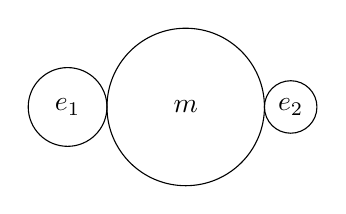
\begin{tikzpicture}
        \draw (0,0) circle (1cm) node {$m$};
        \draw (-1.5,0) circle (0.5cm) node {$e_1$};
        \draw (1.33333,0) circle (0.3333333cm) node {$e_2$};
    \end{tikzpicture}
\end{figure}

\noindent These two encoders are geared at different ratios to the mechanism.

If the rates are "coprime" --- that is, you can't just multiply one encoder ratio by some integer to get the other ratio, then the readings from these two encoders could be combined to give additional information about where the end mechanism is positioned. 

Them being coprime is important, as otherwise you intuitively don't get more information. For example, if your two encoders rotate 2x and 4x as fast as the main mechanism, then with just the 2x reading you can determine exactly where a 4x reading would be -- you take the 2x reading modulo half its range.

The amount of rotation one can uniquely determine to some position is limited by how many rotations your mechanism can go before both encoders end up in the same spot again.

E.g. if both encoder readings both start at $(e_1, e_2) = (0, 0)$, then the number of mechanism rotations it takes for both of them to read $(e_1 = 0, e_2 = 0)$ again is the number of rotations our CRT setup will work for, as we've reached a point at which we can't disambiguate. (Are we at 0 degrees or at 760 degrees? We don't know.)

You also want these ratios to be, well, \textit{rational}, at least to each other.
Sensor ratios of $r_1 = \pi$ and $r_2 = 2$ for example just aren't gonna work; 
while the idea of "well, there's no least common multiple" seems compelling, you quickly run into issues with the CRT just not working at all for this and your encoder ticks having finite precision.
Proving the non-functionality of irrational ratios here is left as an exercise to the reader, because it's outside of the scope of this document.
You probably shouldn't be using smooth belts or weird linkages for measurement encoder axles anyway.

\section{Definitions of variables and symbols}

Let's first define some symbols used throughout.

To represent movement, we will use rotations or revolutions, and we are assuming a setup with two encoders geared at coprime ratios to a mechanism.

\begin{itemize}
    \item $\mathbb{Q}$ represents the set of all rational numbers and $\mathbb{Q^+}$ restricts this to positive rationals.
    \item $\mathbb{Z}$ represents the set of all integers and $\mathbb{Z^+}$ restricts this to positive integers.
    \item $[0, 1)$ is the set of values from 0 inclusive to 1 exclusive. For our purposes we'll just say these are all rational values, which in practice they will be.
    \item $\in$ is the "contains" symbol, and signifies that a value belongs to a set.
    \item The mechanism we are trying to measure will at any given point be rotated $m$ rotations.
    \item $e_1 \in [0, 1)$ represents the sensor reading of encoder 1 in rotations, and wraps around at 1 rotation. 
    \item $e_2 \in [0, 1)$ represents the sensor reading of encoder 2 in rotations, and wraps around at 1 rotation.
    \item $r_1 \in \mathbb{Q^+}$ is the gear ratio between the mechanism and encoder 1.
    \item $r_2 \in \mathbb{Q^+}$ is the gear ratio between the mechanism and encoder 2. For each single positive revolution of the mechanism, encoder 2 will rotate in the positive direction 2 times.
    \item $i_1 > 0, i_2 > 0 \in \mathbb{Z}$ represent the integer number of full rotations encoders 1 and 2 have moved.
    \item We assume that if $m = 0$, then $i_1 = i_2 = 0$ and $e_1 = e_2 = 0$ as well. 
\end{itemize}

The values of $r_1$ and $r_2$ can be anything, and we could even extend this paper to have more than two encoders, but in worked examples we will generally define:

\begin{itemize}
    \item $r_1 = 1.5$ such that for each single positive revolution of the mechanism, encoder 1 will rotate in the positive direction 1.5 times.
    \item $r_2 = 2$ such that for each single positive revolution of the mechanism, encoder 1 will rotate in the positive direction 2 times.
\end{itemize}

\subsection{Relating these values to each other}

We can set up some equations that govern the system by using the ratios $r_1$ and $r_2$ to convert the mechanism position $m$ to encoder rotations.

\begin{align*}
    r_1m &= i_1 + e_1\\
    r_2m &= i_2 + e_2\\
\end{align*}

We break down each encoder's movement into an integer portion $i_i$ representing full rotations and a fractional portion $e_i$ representing what the encoder tells us.

\subsection{Coordinate system advice}

My advice is if you use some other turret coordinate system (e.g. one with negative numbers), make your startup absolute position measurements in CRT-land first (with all non-negative rotations from 0 to whatever) and then convert them to your favorite rotational reference system; due to how critical it is that encoders stay synched, you should generally only use CRT measurements to pre-seed continuous multi-turn measurements for active control use anyway.

\section{Deriving the range of motion}

Before we even touch the remainder theorem stuff, we gotta know the range of motion that we can uniquely determine a position given our gear ratios first.
This is critical as it determines what gear ratios mechanical team needs to install with regards to ones encoders for a turret or whatever.

From a mathematical perspective, it's important too, because it sets an upper bound on what we can do to find mechanism positioning.

\subsection{Does a period exist?}

Let's start with this statement.

\begin{theorem}
    The maximum uniquely determinable range of motion is the minimum distance between instances where the encoders read $(e_1 = 0, e_2 = 0)$, or, in essence, the period of our measurements.
\end{theorem}

\noindent Hold on.  Does a period actually \textit{exist?}
That is, if we rotate our mechanism $m$, will there be a spot where $e_1$ and $e_2$ read the same thing again?

\subsubsection{It does.}

Assume it didn't for a moment, and that once you start increasing $m$ then $e_1 \neq e_2$.
This implies that there does not exist some $m$ where $e_p = e_1 = e_2 \mid m > 0$. 
Let's see how this works with our system equations:

\begin{align*}
    r_1m &= i_1 + e_1\\
    r_2m &= i_2 + e_2\\
    m &= \frac{1}{r_1}(i_1 + e_1) = \frac{1}{r_2}(i_2 + e_2)\\
\end{align*}

\noindent Let's get rid of $m$ and migrate all the $e_i$ to one side and $i_i$ to the other.

\begin{align*}
    r_1(i_2 + e_2) &= r_2(i_1 + e_1)\\
    r_1i_2 + r_1e_2 &= r_2i_1 + r_2e_1\\
    r_1i_2 - r_2i_1 &= r_2e_1 - r_1e_2\\
    \frac{r_1}{r_2}i_2 - i_1 &= e_1 - \frac{r_1}{r_2}e_2 \\
\end{align*}

Since $r_1$ and $r_2$ are positive rational numbers, we can represent them in terms of, well, \textit{ratios}, of positive integers that when mixed together also produce a positive value:

\begin{align*}
    r_1 &= \frac{n_1}{d_1} \mid n_1, d_1 \in \mathbb{Z^+}\\
    r_2 &= \frac{n_2}{d_2} \mid n_2, d_2 \in \mathbb{Z^+}\\
    r_1/r_2 &= \frac{n_1d_2}{n_2d_1} > 0\\
\end{align*}

And if we just select our $i_1$ and $i_2$ to some of these decomposed values (whose values and products by construction are guarenteed to be positive integers) we get something interesting:
\begin{align*}
    i_2 &= n_2d_1 > 0\\
    i_1 &= n_1d_2 > 0\\
    \implies \frac{r_1}{r_2}i_2 - i_1 &= \frac{n_1d_2}{n_2d_1}n_2d_1 - n_1d_2\\
    &= n_1d_2 - n_1d_2 = 0\\
    \implies e_1 - \frac{r_1}{r_2}e_2 &= 0\\
    e_1 &= \left.\frac{r_1}{r_2}e_2 \right| \frac{r_1}{r_2} > 0\\
    \implies e_1 &= e_2\\
\end{align*}

This is a \textbf{proof by contradiction.} We assumed that $e_1 \neq e_2$ would be true for all positive values of $m, i_1, i_2$, but we constructed one where they have to be equal by selecting specific $i_1$ and $i_2$. 


\subsection{Okay but what's the \textit{minimum} range?}


To find the minimum number of non-zero mechanism rotations $m_{max} > 0$ at which $(e_1, e_2) = (0, 0)$, we need to find the smallest mechanism rotation value such that encoders 1 and 2 have both rotated some exact integer number of rotations.

After all, at an exact integer number of rotations upon encoder 1, $e_1 = 0$, and likewise for encoder 2.
These could be any integer number of rotations, but we're looking for some specific (minimum) positive values.

As such, let's call these integers $i_1 \in \mathbb{Z^+}$ and $i_2 \in {\mathbb{Z^+}}$ as some exact number of rotations on encoder 1 and 2 respectively. 
To find the first point at which we get a $(e_1 = 0, e_2 = 0)$ wraparound, we need to find the \textbf{smallest positive values} of $i_1$ and $i_2$ where 

\[
    m_{max} = i_1 / r_1 = i_2 / r_2
\]

as $i_1$ and $i_2$ represent number of encoder rotations, so dividing them by the gear ratio yields mechanism rotations.

Let's do some rearranging, then, shall we?

\begin{align*}
    \frac{i_1}{r_1} &= \frac{i_2}{r_2}\\
    \frac{i_1}{i_2} &= \frac{r_1}{r_2}\\
\end{align*}

The smallest integer values for $i_1$ and $i_2$ are going to be the numerator and denominator you get by simplifying the fraction $\frac{r_1}{r_2}$, because a simplified fraction by definition is where your numerator and denominator are coprime to each other; that is, they do not share any prime factors.

To simplify the fraction and remove the prime factors, we divide both $r_1$ and $r_2$ by their greatest common denominator (GCD), and thus we can state:

\begin{align*}
    i_1 &= r_1 / \gcd(r_1, r_2)\\
    i_2 &= r_2 / \gcd(r_1, r_2)\\
\end{align*}

The GCD can be tricky to reason about with gear ratios that can be rational (e.g. 1.5), so we can define $\gcd(r_1, r_2)$ as the largest value where $r_1 / \gcd(r_1, r_2)$ and $r_2 / \gcd(r_1, r_2)$ are both positive integers. E.g. for $r_1 = 1.5, r_2 = 2$, then:

\begin{align*}
    \gcd(r_1, r_2) &= \gcd(1.5, 2)\\
    1.5 / \gcd(1.5, 2) &\in \mathbb{Z^+}\\
    2 / \gcd(1.5, 2) &\in \mathbb{Z^+}\\
    1.5 / 0.5 &= 3\\
    2 / 0.5 &= 4\\
    \gcd(r_1, r_2) &= 0.5\\
\end{align*}

Now I basically calculated this off of vibes, so a more practical approach in software is to derive the GCD via the least common multiple (LCM), and you can compute the LCM for rational numbers by multiplying $r_1$ by each positive integers until the product is cleanly divisible by $r_2$ without any remainder. 

\begin{align*}
    r_1 &= 1.5\\r_2 &= 2\\
    \lcm(r_1, r_2) &= \lcm(1.5, 2)\\
    (1.5 * 1) \mod 2 &= 0.5 \neq 0\\
    (1.5 * 2) \mod 2 &= 1 \neq 0\\
    &\vdots\\
    (1.5 * 4) \mod 2 &= 0\\
    \lcm(r_1, r_2) &= 1.5 * 4 = 6\\
    \gcd(r_1, r_2) &= \frac{r_1r_2}{\lcm(r_1, r_2)} = \frac{1.5 * 2}{6}= \frac{1}{2}\\
\end{align*}

Circling back to our equations, we then plug in our values to derive $i_1$ and $i_2$ to see that they are in fact coprime integers:

\begin{align*}
    i_1 &= r_1 / \gcd(r_1, r_2) = 1.5 / 0.5 = 3\\
    i_2 &= r_2 / \gcd(r_1, r_2) = 2 / 0.5 = 4\\
\end{align*}

We can see that if you calculate how much the mechanism moves under $i_1$ rotations of encoder 1 or $i_2$ rotations of encoder 2 that they are both equal:

\begin{align*}
    m &= i_1 / r_1 = 3 / 1.5 = 2\\
    &= i_2 / r_2 = 4 / 2 = 2\\
\end{align*}

As such, our range of motion $m_{max}$ in our example is \textbf{2 mechanism rotations.}

\section{Okay where does the Chinese factor into this}

Across our $m_{max} = 2$ rotations of range, we can look at how many rotations each encoder will go within said range.
Encoder 1 will go $2 * r_1 = 3$ rotations, while encoder 2 will go $2 * 2 = 4$ rotations, and we can think of each of these encoder rotations as sub-regions.

\begin{figure}[ht]
    \center
    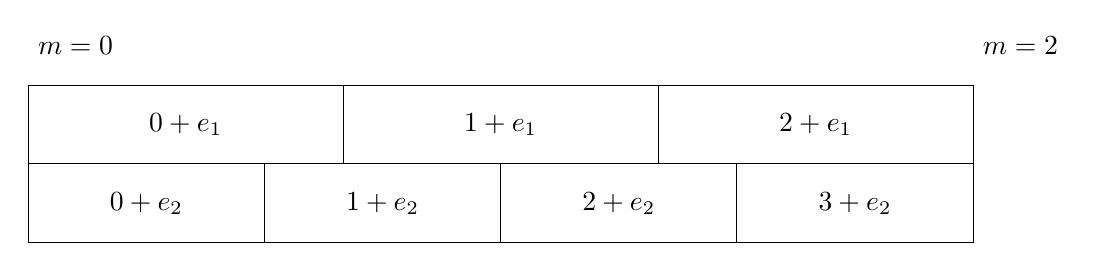
\begin{tikzpicture}
        \draw (0, 2.5) node[anchor=west]{$m = 0$};
        \draw (12, 2.5) node[anchor=west]{$m = 2$};
        \draw [draw=black] (0, 1) rectangle ++(4,1) node[midway] {$0 + e_1$};
        \draw [draw=black] (4, 1) rectangle ++(4,1) node[midway] {$1 + e_1$};
        \draw [draw=black] (8, 1) rectangle ++(4,1) node[midway] {$2 + e_1$};

        \draw [draw=black] (0, 0) rectangle ++(3,1) node[midway] {$0 + e_2$};
        \draw [draw=black] (3, 0) rectangle ++(3,1) node[midway] {$1 + e_2$};
        \draw [draw=black] (6, 0) rectangle ++(3,1) node[midway] {$2 + e_2$};
        \draw [draw=black] (9, 0) rectangle ++(3,1) node[midway] {$3 + e_2$};
    \end{tikzpicture}
\end{figure}

With the LCM of the number of sub-regions for each encoder $\lcm(3, 4) = 12$, we can delineate sub-regions for each combination of encoder 1 and encoder 2's possible rotations. These sub-regions cleanly divide up the rotations of encoders 1 and 2 -- these are 4 of them to an $e_1$ rotation and 3 of them to an $e_2$ rotation.


\begin{figure}[ht]
    \center
    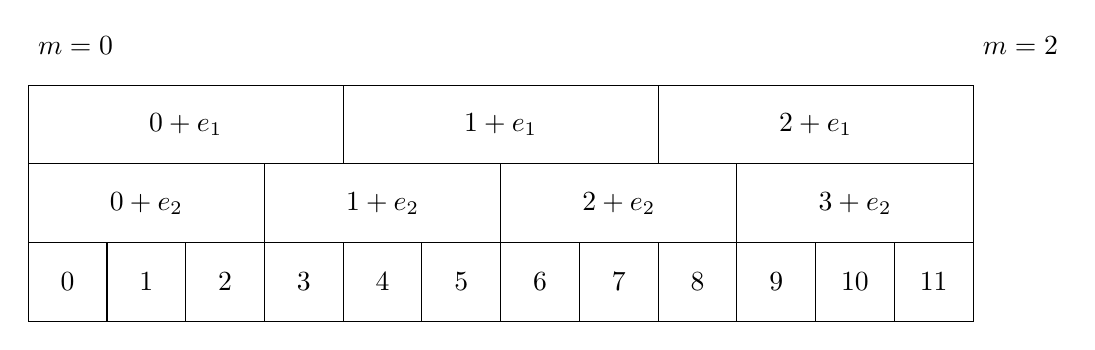
\begin{tikzpicture}
        \draw (0, 3.5) node[anchor=west]{$m = 0$};
        \draw (12, 3.5) node[anchor=west]{$m = 2$};
        \draw [draw=black] (0, 2) rectangle ++(4,1) node[midway] {$0 + e_1$};
        \draw [draw=black] (4, 2) rectangle ++(4,1) node[midway] {$1 + e_1$};
        \draw [draw=black] (8, 2) rectangle ++(4,1) node[midway] {$2 + e_1$};

        \draw [draw=black] (0, 1) rectangle ++(3,1) node[midway] {$0 + e_2$};
        \draw [draw=black] (3, 1) rectangle ++(3,1) node[midway] {$1 + e_2$};
        \draw [draw=black] (6, 1) rectangle ++(3,1) node[midway] {$2 + e_2$};
        \draw [draw=black] (9, 1) rectangle ++(3,1) node[midway] {$3 + e_2$};

        \draw [draw=black] (0, 0) rectangle ++(1,1) node[midway] {0};
        \draw [draw=black] (1, 0) rectangle ++(1,1) node[midway] {1};
        \draw [draw=black] (2, 0) rectangle ++(1,1) node[midway] {2};
        \draw [draw=black] (3, 0) rectangle ++(1,1) node[midway] {3};
        \draw [draw=black] (4, 0) rectangle ++(1,1) node[midway] {4};
        \draw [draw=black] (5, 0) rectangle ++(1,1) node[midway] {5};
        \draw [draw=black] (6, 0) rectangle ++(1,1) node[midway] {6};
        \draw [draw=black] (7, 0) rectangle ++(1,1) node[midway] {7};
        \draw [draw=black] (8, 0) rectangle ++(1,1) node[midway] {8};
        \draw [draw=black] (9, 0) rectangle ++(1,1) node[midway] {9};
        \draw [draw=black] (10, 0) rectangle ++(1,1) node[midway] {10};
        \draw [draw=black] (11, 0) rectangle ++(1,1) node[midway] {11};
    \end{tikzpicture}
\end{figure}
\newpage

\subsection{Deriving the $e_1$ field}

These sub-regions will let us apply the Chinese Remainder Theorem, as we can see some modulo stuff going on.

First, notice how each rotation of $e_1$ covers exactly four sub-regions:

\begin{figure}[ht]
    \center
    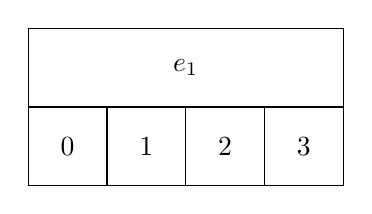
\begin{tikzpicture}
        \draw [draw=black] (0, 1) rectangle ++(4,1) node[midway] {$e_1$};
        \draw [draw=black] (0, 0) rectangle ++(1,1) node[midway] {0};
        \draw [draw=black] (1, 0) rectangle ++(1,1) node[midway] {1};
        \draw [draw=black] (2, 0) rectangle ++(1,1) node[midway] {2};
        \draw [draw=black] (3, 0) rectangle ++(1,1) node[midway] {3};
    \end{tikzpicture}
\end{figure}

To derive the which of the four possible sub-region indexes for some encoder reading $e_1$, we might do

\[
    x = \lfloor e_1 * 4 \rfloor \pmod{4}
\]

where $e_1$ is once again a reading between $[0.0\dots1.0)$ rotations and $\lfloor x \rfloor$ is a floor function.

\subsection{Deriving the $e_2$ field}

You can also do this for $e_2$ as well:

\begin{figure}[ht]
    \center
    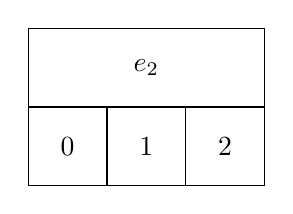
\begin{tikzpicture}
        \draw [draw=black] (0, 1) rectangle ++(3,1) node[midway] {$e_2$};
        \draw [draw=black] (0, 0) rectangle ++(1,1) node[midway] {0};
        \draw [draw=black] (1, 0) rectangle ++(1,1) node[midway] {1};
        \draw [draw=black] (2, 0) rectangle ++(1,1) node[midway] {2};
    \end{tikzpicture}
\end{figure}

\[
    x = \lfloor e_2 * 3 \rfloor \pmod{3}
\]

\subsection{Formulating the CRT problem so we can say there's a solution}

We know $e_1$ and $e_2$ given they're our encoder readings. 
We're trying to find $x \in [0\dots11]$ as it can be used to derive our multi-turn position.
As such, we can state the following:

\begin{align*}
    x &\equiv \lfloor e_1 * 4 \rfloor \pmod{4}\\
    x &\equiv \lfloor e_2 * 3 \rfloor \pmod{3}\\
\end{align*}

Since the moduli are coprime with each other (downstream of the gear ratios being coprime), we can cite the Chinese Remainder Theorem to state that a unique value of $x$ must exist for every possible combination of $\lfloor e_1 * 4 \rfloor$ and $\lfloor e_2 * 3 \rfloor$. 


I'm not really here to prove why the Chinese Remainder Theorem works, but I haven't really seen much showing why it's even applicable to the problem to begin with, so here we are.
Learning why the CRT holds true is an exercise left for the reader, and I was too mid at college math and explaining new concepts in general to help you out here.

I am a believer in seeing is believing, though, and you can see that on the diagram on the previous page that there's unique positions within each encoder 1 and 2 rotation for each of the 12 sub-sections.

\section{Okay how do I calculate all this stuff}

\subsection{I'm not a math wiz how do i find $x$ to begin with}

\subsection{Going from $x$ to $m$}

Once we calculate our $x$, we can determine our mechanism rotations $m$, as knowing $x$ means you know how many full rotations $e_1$ or $e_2$ has made and you can just add on their readings and convert to mechanism rotations to get your position:

\begin{align*}
    m &= \left(\frac{x}{3} + e_1\right) * r_1\\
    &= \left(\frac{x}{4} + e_2\right) * r_2\\
\end{align*}

\end{document}
